
\documentclass[tikz]{standalone}
\usepackage{lib/basic}
\tikzset{
Line/.style={draw=black, ->, line width=1.5pt},
}
\begin{document}
\begin{tikzpicture}[]\node at (0, 0){\begin{tikzpicture}
        \coordinate (p) at (0,0);\draw[step=1, ultra thick, color=black, fill=black!25!white, draw=black, shift={(p)}] (0, 0) grid (5, -5)foreach[count=~] \l in {1, 2, 3, 4, 5, 6, 7, 8, 9, 10, 11, 12, 13, 14, 15, 16, 17, 18, 19, 20, 21, 22, 23, 24, 25} {({0.5+mod(~-1,5}, {-0.5-div(~-1,5}) node {\Large \l}};
	\node[align=center, text width=50pt, yshift = 10pt, xshift=2pt, right of=p] (2) {};\end{tikzpicture}};\node at (5, 0){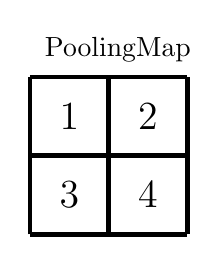
\begin{tikzpicture}
        \coordinate (p) at (0,0);\draw[step=1, ultra thick, color=black, fill=black!25!white, draw=black, shift={(p)}] (0, 0) grid (2, -2)foreach[count=~] \l in {1, 2, 3, 4} {({0.5+mod(~-1,2}, {-0.5-div(~-1,2}) node {\Large \l}};
	\node[align=center, text width=50pt, yshift = 10pt, xshift=2pt, right of=p] (3) {PoolingMap};\end{tikzpicture}};\node at (10, 0){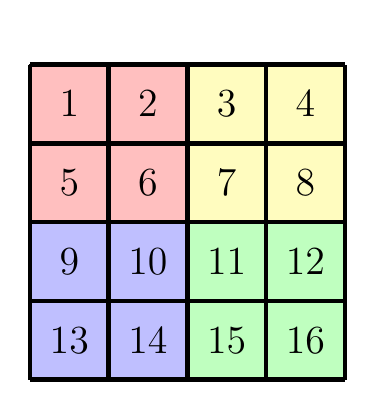
\begin{tikzpicture}
        \coordinate (p) at (0,0);\draw[shift={(0, 0)}, fill=red!25!white] (0, 0) rectangle (2, -2);
\draw[shift={(0, 0)}, fill=yellow!25!white] (2, 0) rectangle (4, -2);
\draw[shift={(0, 0)}, fill=blue!25!white] (0, -2) rectangle (2, -4);
\draw[shift={(0, 0)}, fill=green!25!white] (2, -2) rectangle (4, -4);
\draw[step=1, ultra thick, color=black, fill=black!25!white, draw=black, shift={(p)}] (0, 0) grid (4, -4)foreach[count=~] \l in {1, 2, 3, 4, 5, 6, 7, 8, 9, 10, 11, 12, 13, 14, 15, 16} {({0.5+mod(~-1,4}, {-0.5-div(~-1,4}) node {\Large \l}};
	\node[align=center, text width=50pt, yshift = 10pt, xshift=2pt, right of=p] (4) {};\end{tikzpicture}};
\draw[Line] (12.5,0) -- (15,0);\node at (17.5, 0){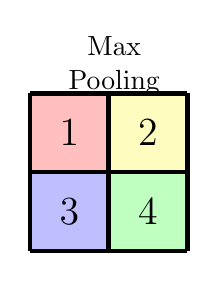
\begin{tikzpicture}
        \coordinate (p) at (0,0);\draw[shift={(0, 0)}, fill=red!25!white] (0, 0) rectangle (1, -1);
\draw[shift={(0, 0)}, fill=yellow!25!white] (1, 0) rectangle (2, -1);
\draw[shift={(0, 0)}, fill=blue!25!white] (0, -1) rectangle (1, -2);
\draw[shift={(0, 0)}, fill=green!25!white] (1, -1) rectangle (2, -2);
\draw[step=1, ultra thick, color=black, fill=black!25!white, draw=black, shift={(p)}] (0, 0) grid (2, -2)foreach[count=~] \l in {1, 2, 3, 4} {({0.5+mod(~-1,2}, {-0.5-div(~-1,2}) node {\Large \l}};
	\node[align=center, text width=50pt, yshift = 10pt, xshift=2pt, right of=p] (5) {Max Pooling};\end{tikzpicture}};
\end{tikzpicture}
\end{document}